\section{Scope and conventions}

\subsection{Purpose}
This document describes the steady-state power flow of a point-to-point HVDC
link: Assuming the power to be defined at the AC terminal of the receiving end. Two HVDC topologies 
arrangements are covered --- the \textbf{symmetrical
monopole (SMP)} and the \textbf{bipole with a dedicated metallic return (BIP)}.

\subsection{Direction and reference conventions}
Power flows from the \textbf{rectifier} (sending station) to the
\textbf{inverter} (receiving station). Four conventions fix the problem:

\begin{enumerate}[label=(\arabic*)]
  \item \textbf{Power is defined at the receiving end}, at the AC terminals of
        the inverter station.
  \item \textbf{DC voltage is regulated at the rectifier DC terminals.} The
        nominal dc voltage $U_{dpe\_rec}$ is defined at the sending station and
        the receiving-end voltage comes out lower by the resistive drop of the line.
  \item \textbf{Converter station losses are a fraction of station throughput}, applied per station, rather than a fixed number of
        megawatts.
  \item \textbf{Conductor resistance is corrected to a design temperature.}
        Conductor data is quoted at 20\,$^{\circ}$C; the flow is evaluated at a
        conductor temperature stated separately, 75\,$^{\circ}$C by default.
\end{enumerate}

Conventions (1) and (2) sit at opposite ends of the line, which is what makes
the current an implicit rather than an explicit quantity: the sending-end power
depends on the line loss, the line loss depends on the current, and the current
depends on the sending-end power. Section~\ref{sec:solution} closes that loop
in one step instead of iterating.

\subsection{Conductor data}
The one genuine conversion concerns the conductor data. Conductor tables give
DC resistance per 1000\,ft --- the values used here are the \emph{DC @
20\,$^{\circ}$C} column of the Southwire ACSR bare conductor tables~[1] ---
so the factor
\[
  \frac{5280\ \mathrm{ft/mi}}{1000\ \mathrm{ft}} = 5.28
\]
converts specific resistance to $\Omega$/mi before multiplying by the line
length in miles.

\subsection{Notation}
Figures~\ref{fig:dc-notation} and~\ref{fig:bip-notation} show the signal notation on
the DC side, for the SMP and BIP topologies.

Each quantity carries the station it is measured at, $rec$ or $inv$. In the
bipole it carries the pole as well, $pos$ or $neg$, since each pole has its own
converter pair; the HV conductor and the DMR are distinguished in both the
resistances, $R_{d\_hv}$ and $R_{d\_dmr}$, and the currents, $I_{d\_hv}$ and
$I_{d\_dmr}$; and $U_{dmr}$ is the DMR potential at the station where the return
is not earthed. The relations in the sections that follow use the unqualified
symbol wherever a statement holds for either pole or for either station.

\begin{figure}[!ht]
  \centering
  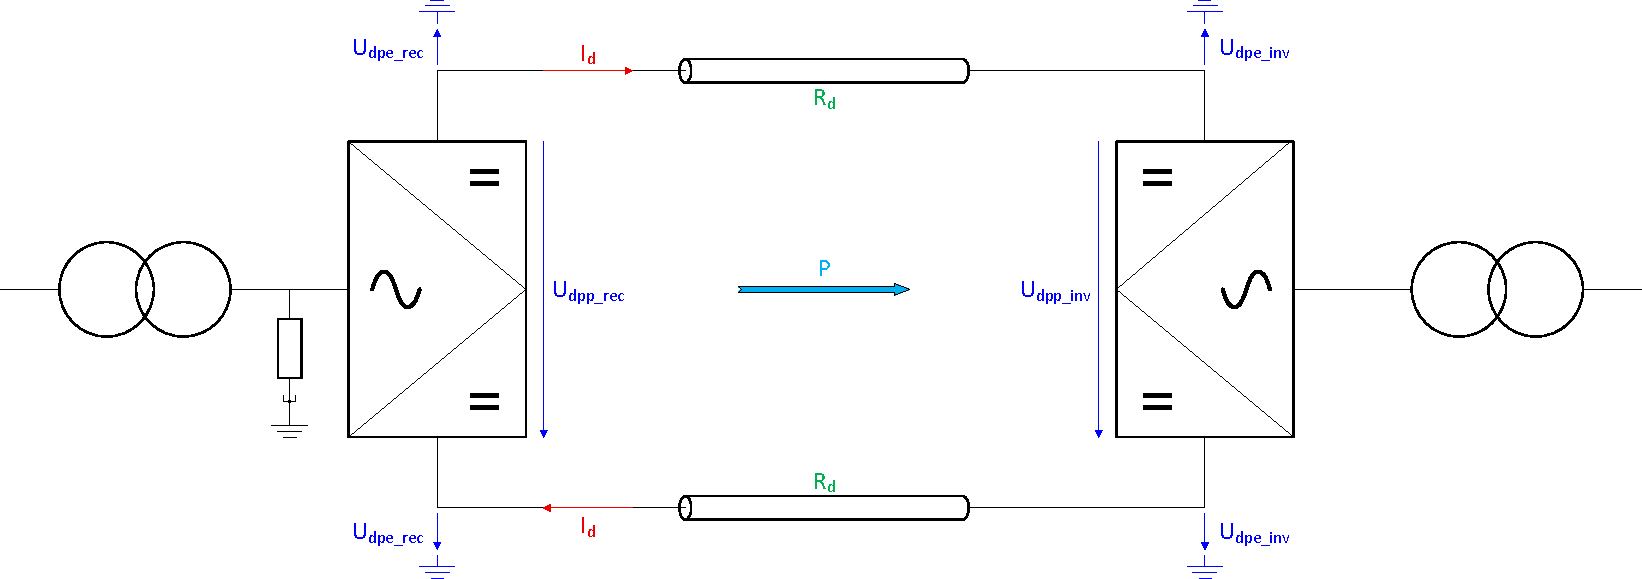
\includegraphics[width=\linewidth]{figures/dc-notation-smp.pdf}
  \caption{DC-side notation for SMP}
  \label{fig:dc-notation}
\end{figure}

\begin{figure}[!ht]
  \centering
  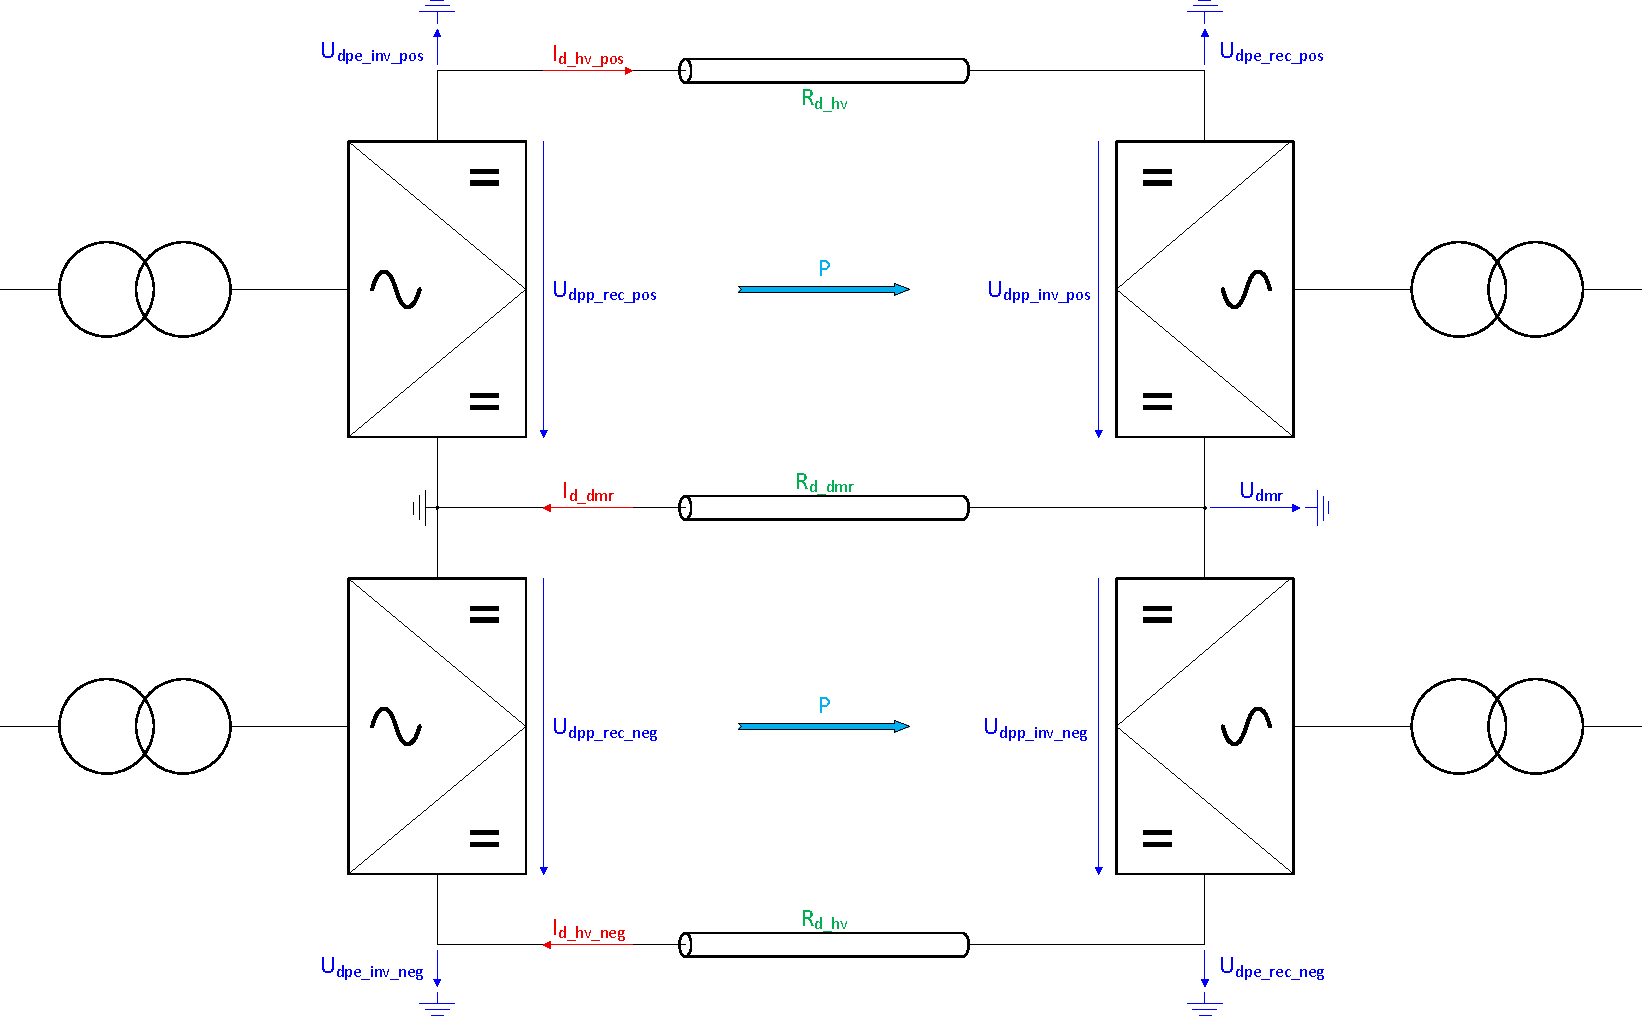
\includegraphics[width=\linewidth]{figures/dc-notation-bip.pdf}
  \caption{DC-side notation for BIP}
  \label{fig:bip-notation}
\end{figure}

\begin{table}[!ht]
  \centering
  \renewcommand{\arraystretch}{1.25}
  \begin{tabularx}{\linewidth}{@{}l l X@{}}
    \toprule
    \multicolumn{1}{c}{\textbf{Symbol}} & \multicolumn{1}{c}{\textbf{Unit}} & \textbf{Quantity} \\
    \midrule
    $P_{ac\_inv}$   & MW            & AC power at the receiving end (inverter AC terminals) --- \emph{given} \\
    $P_{ac\_rec}$   & MW            & AC power drawn at the sending end (rectifier AC terminals) \\
    $P_{dc\_inv}$   & MW            & DC power at the inverter DC terminals \\
    $P_{dc\_rec}$   & MW            & DC power at the rectifier DC terminals \\
    $U_{dpe}$      & kV            & DC pole-to-ground (earth) voltage \\
    $U_{dpe\_rec}$  & kV            & DC pole-to-ground voltage at the rectifier --- \emph{given} \\
    $U_{dpe\_inv}$  & kV            & DC pole-to-ground voltage at the inverter \\
    $U_{dpp}$      & kV            & DC voltage across a converter's DC terminals; $U_{dpp} = 2\cdot U_{dpe}$ for a symmetrical monopole \\
    $U_{dmr}$      & kV            & DMR potential at the station where the return is not earthed \\
    $U_{dpm\_inv}$  & kV            & DC pole-to-DMR voltage at the inverter (one pole out) \\
    $I_{d}$        & kA            & DC pole current, operating value \\
    $k$            & ---           & Number of energised poles: 2 normally, 1 with a pole out \\
    $L$            & mi            & DC line length \\
    $r'_{d\_hv}$      & $\Omega$/1000\,ft & Specific resistance of one HV subconductor \\
    $n_{hv}$       & ---           & Subconductors per pole (bundle count) \\
    $R_{d\_hv}$     & $\Omega$      & Resistance of one pole conductor over the whole length \\
    $r'_{d\_dmr}$     & $\Omega$/1000\,ft & Specific resistance of one DMR subconductor \\
    $n_{dmr}$      & ---           & Subconductors in the DMR bundle \\
    $R_{d\_dmr}$    & $\Omega$      & Resistance of the DMR over the whole length \\
    $I_{d\_dmr}$    & kA            & Current in the DMR; zero when the bipole is balanced \\
    $R_{loop}$     & $\Omega$      & Resistance of the complete current path (out and return) \\
    $T_{ref}$      & $^{\circ}$C   & Temperature the conductor resistance data refers to \\
    $T$            & $^{\circ}$C   & Conductor temperature the flow is evaluated at \\
    $T_{0}$        & $^{\circ}$C   & Inferred zero-resistance temperature of the conductor material \\
    $k_{T}$        & ---           & Temperature correction factor on the specific resistance \\
    $p_{rec}$      & ---           & Rectifier station loss fraction of throughput \\
    $p_{inv}$      & ---           & Inverter station loss fraction of throughput \\
    $P_{loss\_line}$& MW            & Total resistive loss of the DC line \\
    $\eta$         & ---           & Overall AC-to-AC efficiency of the link \\
    \bottomrule
  \end{tabularx}
  \caption{Notation.}
  \label{tab:notation}
\end{table}

\pagebreak
